\documentclass[a4paper,12pt]{article}

\usepackage{mystyle}

\graphicspath{ {images/} }

\usetikzlibrary{arrows.meta}

\definecolor{my-red}{RGB}{176, 0, 0}
\definecolor{my-blue}{RGB}{0, 0, 153}


\author{Алексеев Василий}
\title{Семинар 5}
\date{6 + 10 октября 2022}


\begin{document}
  \maketitle
  
  \tableofcontents

  \thispagestyle{empty}
  
  \newpage
  
  \pagenumbering{arabic}


  \section{Прямая на плоскости}
  
  \begin{figure}[h]
    \centering
    
    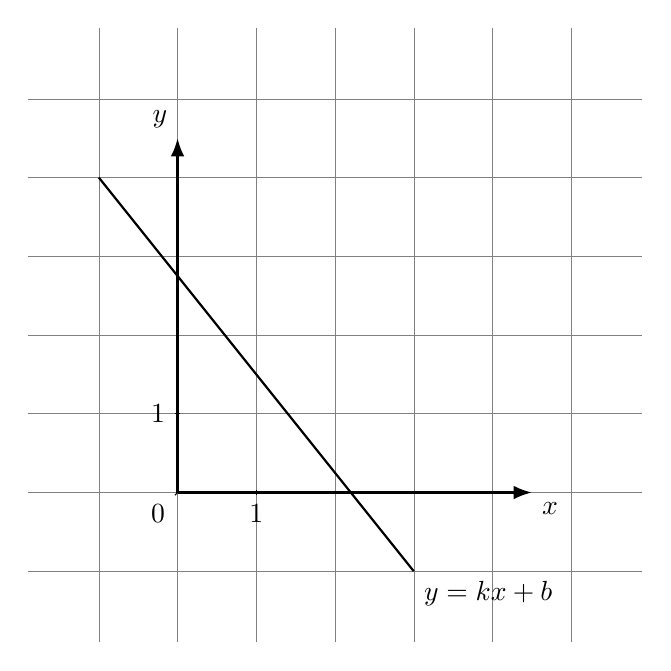
\begin{tikzpicture}
      \draw[step=1cm,gray,very thin] (-1.9,-1.9) grid (5.9,5.9);
      
      \draw[thick,-Latex] (0,0) -- (4.5,0) node[anchor=north west] {$x$};
      \draw[thick,-Latex] (0,0) -- (0,4.5) node[anchor=south east] {$y$};
      
      \draw (0,0) -- (-1pt,-1pt) node[anchor=north east] {$0$};
      
      \foreach \x in {1}
        \draw (\x cm,1pt) -- (\x cm,-1pt) node[anchor=north] {$\x$};
      \foreach \y in {1}
        \draw (1pt,\y cm) -- (-1pt,\y cm) node[anchor=east] {$\y$};
      
      \draw[thick] (-1,4) -- (3,-1) node[anchor=north west] {$y = kx + b$};
    \end{tikzpicture}
    
    \caption{Прямоугольная декартова система координат на плоскости и прямая, заданная в этой системе координат уравнением $y \hm= kx \hm+ b$.}
    \label{fig:line-on-plane}
  \end{figure}
  
  Пусть на плоскости есть прямоугольная система координат (\ref{fig:line-on-plane}).
  Тогда прямая может быть задана уравнением
  \begin{equation}\label{eq:lile-on-plane-school-version}
    y = kx + b
  \end{equation}
  где $k \hm\in \RR$~---~угловой коэффициент (тангенс угла между прямой и положительным направлением оси $X$),
  а $b \hm\in \RR$~---~свободный член (ордината точки пересечения прямой с осью $Y$).
  Уравнение прямой~---~связь между координатами точек, такая что точки прямой и только они удовлетворяют этому соотношению.
  Но с помощью уравнения (\ref{eq:lile-on-plane-school-version})
  нельзя задать вертикальную прямую (параллельную оси $Y$).
  Вертикальные прямые можно описать с помощью уравнения
  \[
    x = x_0
  \]
  где $x_0 \hm\in \RR$.
  Вместо уравнений для двух частных случаев (наклонная прямая и вертикальная) можно рассмотреть уравнение для произвольной прямой на плоскости, включающее в себя описанные частные случаи:
  \begin{equation}\label{eq:line-in-coord-system}
    Ax + By + C = 0,\ A^2 + B^2 \not= 0
  \end{equation}
  
  Отметим, что коэффициенты в уравнении прямой (\ref{eq:line-in-coord-system}) определены с точностью до ненулевого множителя.
  Так, пусть прямая задаётся уравнением
  \[
    Ax + By + C = 0
  \]
  Но тогда и уравнение
  \[
    2Ax + 2By + 2C = 0
  \]
  хоть формально и отличается от первого, но задаёт ту же прямую: если координаты точки удовлетворяют первому уравнению, то они удовлетворяют и второму, и наоборот.
  
  Также стоит подчеркнуть, что коэффициенты в уравнении зависят от выбранной системы координат.
  Так, в некоторой декартовой прямоугольной системе координат $O; \bds e_1, \bds e_2$ уравнение прямой может иметь вид 
  \[
    Ax + By + C = 0
  \]
  а в другой системе координат $O'; \bds e_1', \bds e_2'$ (не обязательно прямоугольной, и базис $e'$ которой не обязательно имеет ту же ориентацию, что и базис $e$) уравнение \emph{той же} прямой может иметь другие коэффициенты
  (координаты обозначим $x', y'$ вместо $x, y$, как координаты в другой декартовой системе):
  \[
    A'x' + B'y' + C' = 0
  \]
  Таким образом, уравнение прямой~---~это способ описания прямой, связанный с выбранной системой координат\footnote{
    В более общем случае, \emph{алгебраическая линия} на плоскости~---~множество точек, определяемых в некоторой декартовой системе координат уравнением
    \begin{equation}\label{eq:algebraic-line}
      A_1 x^{k_1} y^{l_1} + \ldots + A_s x^{k_s} y^{l_s} = 0, \quad k_i, l_i \in \NN_{\geq 0}
    \end{equation}
    
    Степень уравнения (порядок алгебраической линии) определяется как максимальная из сумм:
    \[
      \max{\{k_1 + l_1, \ldots, k_s + l_s\}}
    \]
    (при условии, что в уравнении приведены подобные члены, и числовой коэффициент $A_i$ в соответствующем одночлене с максимальной суммой $k_i \hm+ l_i$ отличен от нуля).

    Существует теорема, согласно которой \emph{алгебраическая линия порядка $p$ на плоскости в \emph{любой} декартовой системе координат может быть задана уравнением вида (\ref{eq:algebraic-line}) порядка $p$}.
    
    При этом свойство неизменности порядка не относится к различным уравнениям, которые линия может иметь в одной и той же системе координат. 
    Например, $x^2 \hm+ y^2 \hm- 1 \hm= 0$ и $(x^2 \hm+ y^2 \hm- 1)^2 \hm= 0$.
  }.
  
  Что можно сказать о прямой по её уравнению?
  Пусть есть прямая $l$, заданная уравнением (\ref{eq:line-in-coord-system}), и точка на прямой $P \hm= (x_0, y_0) \hm\in l$.
  Рассмотрим точку $P' \hm= (x_0 \hm- B, y_0 \hm+ A)$.
  Принадлежит ли она прямой $l$?
  \[
    A (x_0 - B) + B (y_0 + A) + C
    = \bigl(A x_0 + B y_0 + C\bigr) - AB + BA
    = 0 + 0
    = 0
    \Rightarrow P' \in l
  \]
  Очевидно, что и точка $P'' \hm= (x_0 \hm- 2B, y_0 \hm+ 2A)$ также лежит на $l$.
  Таким образом, радиус-вектор любой точки на прямой может быть получен из радиуса-вектора исходной точки $P$ сдвигом вдоль вектора
  \begin{equation}
    \boxed{\bds a = (-B, A)}
  \end{equation}
  который можно взять в качестве \emph{направляющего вектора} прямой, то есть ненулевого вектора, параллельного прямой.
  
  Зная одну точку на прямой и направляющий вектор, можно записать \emph{векторное уравнение прямой в параметрической форме}:
  \begin{equation}\label{eq:line-as-radius-vector}
    \boxed{\bds{r} = \bds{r}_0 + \bds{a} t, \quad \bds{a} \not= \bds{0},\ t \in \RR}
  \end{equation}
  где $\bds r_0$~---~вектор начальной точки на прямой, $\bds a$~---~направляющий вектор, а $t$~---~числовой параметр.
  
  Векторное уравнение равносильно системе из двух скалярных уравнений в общей декартовой системе координат:
  \begin{equation}
    \boxed{\left\{
      \begin{aligned}
        &x = x_0 + \alpha t\\
        &y = y_0 + \beta t
      \end{aligned}
    \right.\quad t \in \RR}
  \end{equation}
  где $(\alpha, \beta) \hm= \bds a$, а потому $\alpha^2 \hm+ \beta^2 \hm{\not=} 0$.
  
  Систему скалярных уравнений, в свою очередь, можно ещё записать в \emph{канонической форме}:
  \[
    \boxed{\frac{x - x_0}{\alpha} = \frac{y - y_0}{\beta}}
  \]
  
  Если система координат \textbf{декартова прямоугольная} (у которой базис ортонормированный), то, зная направляющий вектор прямой $(-B, A)$, можно найти вектор нормали к прямой (\ref{fig:n-perp-a}):
  \[
    (\bds a, \bds n) = -B \cdot n_x + A \cdot n_y = 0 \Rightarrow \bds n \propto (A, B)
  \]
  и в качестве вектора нормали можно взять
  \begin{equation}
    \bds n = (A, B)
  \end{equation}
  
  \begin{figure}[h]
    \centering
    
    \includegraphics[width=0.5\textwidth]{n-perp-a}
    
    \caption{Направляющий вектор $\bds a$ прямой $l$ и вектор нормали $\bds n$ к ней.}
    \label{fig:n-perp-a}
  \end{figure}
  
  Зная вектор нормали $\bds n$ к прямой, можно записать \emph{нормальное векторное уравнение прямой} (принимая во внимание, что $\bds a \hm\perp \bds n$, а $\bds a \hm\parallel (\bds r \hm- \bds r_0)$ для точек $\bds r$ прямой и только для них)
  \begin{equation}
    \boxed{(\bds r - \bds r_0, \bds n) = 0,\quad \bds n \not= \bds 0}
  \end{equation}
  или
  \[
    (\bds r, \bds n) = D,\quad \bds n \not= \bds 0,\ D \in \RR
  \]
  
  Одной из базовых задач является нахождение расстояния от точки до прямой.
  Пусть есть точка $A \hm= (x_1, y_1) \hm= \bds r_1$ и прямая $l$, заданная с помощью радиуса вектора начальной точки $\bds r_0$ и направляющего вектора $\bds a$.
  Тогда расстояние от точки $A$ до прямой $l$ можно найти как модуль векторной проекции вектора $\bds r_1 \hm- \bds r_0$ на направление, определяемое вектором нормали к прямой $\bds n$:
  \begin{equation}
    \boxed{\rho(A, l) = \frac{\bigl|(\bds r_1 - \bds r_0, \bds n)\bigr|}{|\bds n|}}
  \end{equation}
  
  Пусть теперь в \textbf{прямоугольной системе} координат прямая $l$ задана уравнением $Ax \hm+ By \hm+ C \hm= 0$.
  Тогда направляющий вектор прямой $\bds a \hm= (-B, A)$, вектор нормали $\bds n \hm= (A, B)$, а расстояние от точки $A$ до прямой $l$:
  \begin{equation*}
  \begin{split}
    \rho(A, l) &= \frac{\bigl|(\bds r_1 - \bds r_0, \bds n)\bigr|}{|\bds n|}
    = \frac{\bigl|(\bds r_1, \bds n) - (\bds r_0, \bds n)\bigr|}{|\bds n|}\\
    &\xrightarrow{\mbox{ДПСК}} \frac{|Ax_1 + By_1 - (Ax_0 + By_0)|}{\sqrt{A^2 + B^2}}
    \stackrel{\bds r_0 \in l}{=} \frac{|Ax_1 + By_1 + C|}{\sqrt{A^2 + B^2}}
  \end{split}
  \end{equation*}
  где \emph{ДПСК}~---~декартова прямоугольная система координат.
  То есть в итоге
  \begin{equation}
    \rho(A, l) = \frac{|Ax_1 + By_1 + C|}{\sqrt{A^2 + B^2}}
  \end{equation}


  \section{Задачи}
  
  \subsection{\# 5.1}
  
  \begin{problem}
    При каком необходимом и достаточном условии прямые $\bds r \hm= \bds r_1 \hm+ \bds a_1 t$ и $\bds r \hm= \bds r_2 \hm+ \bds a_2 t$
    \begin{enumerate}
      \item Пересекаются в единственной точке?
      \item Параллельны, но не совпадают?
      \item Совпадают?
    \end{enumerate}
  \end{problem}
  
  \begin{solution}
    \begin{figure}[h]
      \centering
      
      \includegraphics[width=0.5\textwidth]{lines-on-plane}
      
      \caption{Варианты взаимного расположения двух прямых на плоскости.}
      \label{fig:lines-on-plane}
    \end{figure}
    
    Рассмотрим пункты по порядку (\ref{fig:lines-on-plane}).
    
    \begin{enumerate}
      \item Очевидно, необходимое и достаточное условие~---~чтобы $\bds a_1$ и $\bds a_2$ были неколлинеарны\footnote{Более строго это можно обосновать, рассмотрев систему уравнений $\bds r_1 \hm+ \bds a_1 t_1 \hm= \bds r_2 \hm+ \bds a_2 t_2$. Если определитель системы отличен от нуля, то, по теореме Крамера, решение существует и единственно. Обратно, если определитель системы равен нулю, то можно показать, что решений либо нет, либо их бесконечно много.}.
      То есть условие
      \[
        \bds a_1 \not\parallel \bds a_2
      \]
      
      \item Первое условие~---~чтобы направляющие векторы были параллельны.
      Но этого недостаточно: надо ``отсечь'' случай совпадения прямых.
      При $\bds a_1 \hm\parallel \bds a_2$ необходимым и достаточным условием совпадения прямых является наличие хотя бы одной общей точки $\bds r_{\star}$.
      Но тогда получаем $\bds r_{\star} \hm= \bds r_1 \hm+ \bds a_1 t_1$ и $\bds r_{\star} \hm= \bds r_2 \hm+ \bds a_2 t_2$, а потому для того, чтобы прямые были различны, должно выполняться $(\bds r_1 \hm- \bds r_2) \hm{\not\parallel} \bds a_1$.
      Итого
      \[
        \left\{
          \begin{aligned}
            &\bds a_1 \parallel \bds a_2\\
            &(\bds r_1 \hm- \bds r_2) \not\parallel \bds a_1
          \end{aligned}
        \right.
      \]
      
      \item Последний случай получается изменением второго условия в предыдущем пункте на противоположное:
      \[
        \left\{
          \begin{aligned}
            &\bds a_1 \parallel \bds a_2\\
            &(\bds r_1 \hm- \bds r_2) \parallel \bds a_1
          \end{aligned}
        \right.
      \]
    \end{enumerate}
  \end{solution}
  
  
  \subsection{\# 5.2(1)}
  
  \begin{problem}
    Найти угол между прямыми $l_1$ и $l_2$, заданными следующими уравнениями:
    \[
      l_1\colon \bds r = \bds r_1 + \bds a_1 t
    \]
    \[
      l_2\colon \bds r = \bds r_2 + \bds a_2 t
    \]
  \end{problem}
  
  \begin{solution}
    Очевидно, угол между прямыми можно найти с помощью направляющих векторов.
    (Направляющие векторы $\bds a_1$ и $\bds a_2$, а также начальные точки прямых $\bds r_1$ и $\bds r_2$ известны по условию.)
    \[
      \cos \angle (\bds a_1, \bds a_2) = \frac{(\bds a_1, \bds a_2)}{|\bds a_1| |\bds a_2|}
    \]
    
    Тогда для угла между прямыми (который считается острым) получаем:
    \[
      \cos \angle (l_1, l_2) = \bigl|\cos \angle (\bds a_1, \bds a_2)\bigr| = \left| \frac{(\bds a_1, \bds a_2)}{|\bds a_1| |\bds a_2|} \right|
    \]
  \end{solution}
  
  
  \subsection{\# 5.9(4)}
  
  \begin{problem}
    Составить уравнение прямой, проходящей через две точки $P(1, -3)$ и $Q(3, -3)$.
  \end{problem}
  
  \begin{solution}
    \leavevmode
    
    \emph{Способ 1 (уравнение в ОДСК).}
    Ищем уравнение прямой в виде:
    \begin{equation}\label{eq:line-in-5-9-4}
      Ax + By + C = 0,\quad A^2 + B^2 \not= 0
    \end{equation}
    
    Точки $P$ и $Q$ принадлежат прямой.
    Поэтому их координаты удовлетворяют уравнению прямой.
    Объединим в систему эти соотношения:
    \[
      \left\{
        \begin{aligned}
          &A - 3B + C = 0\\
          &3A - 3B + C = 0
        \end{aligned}
      \right.
    \]
    
    Вычитая из одного уравнения другое, находим, что $A \hm= 0$.
    Тогда для поиска оставшихся коэффициентов в уравнении прямой получаем соотношение:
    \[
      -3B + C = 0
    \]
    
    Откуда можно, например, выразить $C$ как $C \hm= 3B$.
    
    Вернёмся к уравнению прямой (\ref{eq:line-in-5-9-4}).
    Получили, что оно должно иметь такой вид:
    \[
      By + 3B = 0
    \]
    
    Можем сократить на $B$, так как этот коэффициент точно не ноль.
    Итоговое уравнение прямой:
    \[
      y + 3 = 0
    \]
    
    \medskip
    
    \emph{Способ 2 (``наблюдение'').}
    Можно заметить, что прямая $PQ$ параллельна оси $X$ (но не факт, что перпендикулярна оси $Y$! только если система координат прямоугольная), причём пересекает ось $Y$ в точке с ординатой $-3$.
    Таким образом, уравнение прямой: $y \hm= -3$.
    
    \medskip
    
    \emph{Способ 3 (векторный параметрический).}
    В качестве направляющего вектора прямой можно взять вектор $\vv{PQ}(2, 0)$.
    Если в качестве начальной точки прямой выбрать точку $P$, то можно записать такое векторное уравнение прямой:
    \[
      \begin{pmatrix}
        x\\y
      \end{pmatrix} = \begin{pmatrix}
        1\\-3
      \end{pmatrix} + \begin{pmatrix}
        2\\0
      \end{pmatrix} t
    \]
    
    Снова получаем, что прямая определяется уравнением $y \hm= -3$.
  \end{solution}
  
  
  \subsection{\# 5.5(2)}
  
  \begin{problem}
    Найти расстояние от точки $M_0(\bds r_0)$ до прямой $l$, заданной уравнением $\bds r \hm= \bds r_1 \hm+ \bds a t$.
  \end{problem}
  
  \begin{solution}
    Пусть $\bds r_x$~---~радиус-вектор ортогональной проекции точки $M_0$ на прямую $l$.
    Тогда
    \[
      \left\{
        \begin{aligned}
          &\bds r_x = \bds r_1 + \bds a \tau\\
          &(\bds r_x - \bds r_0) \perp \bds a
        \end{aligned}
      \right.
    \]
    При этом $(\bds r_x \hm- \bds r_0) \hm\perp \bds a$ равносильно $(\bds r_x \hm- \bds r_0, \bds a) \hm= 0$.
    Подставляя $\bds r_x$ из первого уравнения системы в скалярное произведение, получаем
    \[
      (\bds r_1 + \bds a \tau - \bds r_0, \bds a) = 0
    \]
    
    Откуда
    \[
      \tau = \frac{(\bds r_0 - \bds r_1, \bds a)}{|\bds a|^2}
    \]
    
    И вектор $\bds r_x$ равен
    \[
      \bds r_x = \bds r_1 + \frac{(\bds r_0 - \bds r_1, \bds a)}{|\bds a|^2} \bds a
    \]
    
    Искомое же расстояние
    \[
      \rho(M_0, l) = |\bds r_x - \bds r_0|
      = \left|\frac{(\bds r_1 - \bds r_0)|\bds a|^2 - \bds a (\bds r_1 - \bds r_0, \bds a)}{|\bds a|^2}\right|
    \]
    
    Получили расстояние от точки до прямой.
    
    Можно заметить, что числитель в последней дроби ``похож'' на развёрнутый ``бац минус цаб''...
    Действительно, можно записать
    \[
      (\bds r_0 - \bds r_1, \bds a) = [\bds a, [\bds r_1 - \bds r_0, \bds a]]
    \]
    но при этом надо сказать, что мы \textbf{с плоскости выходим в пространство} с некоторым базисом (при этом в данном случае не важно, как ориентирован базис в пространстве, как векторы базиса в пространстве расположены по отношению к исходной плоскости, где лежат прямая $l$ и точка $M_0$).
    Итого, с помощью векторного произведения запись для расстояния можно записать в более компактном виде:
    \[
      \rho(M_0, l) = \frac{\Bigl|\bigl[\bds a, [\bds r_1 - \bds r_0, \bds a]\bigr]\Bigr|}{|\bds a|^2}
      = \frac{\bigl|[\bds r_1 - \bds r_0, \bds a]\bigr|}{|\bds a|}
    \]
    
    На самом деле эту формулу можно бы было получить и сразу, без ``озарения с ``бац минус цаб''.
    Ведь в числителе стоит площадь параллелограмма, построенного на векторах $\bds r_1 \hm- \bds r_0$ и $\bds a$, а в знаменателе~---~длина одной из сторон этого параллелограмма.
    Или так: если расписать числитель и сократить дробь на $|\bds a|$, то останется $|\bds r_1 \hm- \bds r_0| \sin \angle(\bds r_1 \hm- \bds r_0, \bds a)$, что и даёт расстояние от точки до прямой.
  \end{solution}
  
  
  \subsection{\# 5.19}
  
  \begin{problem}
    Составить уравнения прямых, проходящих через точку $A(-1, 5)$ и равноудалённых от точек $B(3, 7)$ и $C(1, -1)$.
  \end{problem}
  
  \begin{solution}
    Расстояние от точки до прямой:
    \[
      \rho = \left|\frac{(\bds r_1 - \bds r_0, \bds n)}{|\bds n|}\right|
    \]
    
    Прямая $a$ равноудалена от $B(3, 7)$ и $C(1, -1)$:
    \[
      \frac{\Bigl|\bigl((3, 7) - (-1, 5), \bds n\bigr)\Bigr|}{|\bds n|} = \rho_{a, B}
      = \rho_{a, C}
      = \frac{\Bigl|\bigl((1, -1) - (-1, 5), \bds n\bigr)\Bigr|}{|\bds n|}
    \]
    \[
      \bigl|(4, 2) \cdot \bds n\bigr| = \bigl|(2, -6) \cdot \bds n\bigr|
    \]
    
    Но не понятно, что с этим делать дальше, потому что система координат может быть и не прямоугольная!
    При вычислении скалярного произведения недостаточно лишь перемножать соответствующие координаты, надо считать ``по-честному'':
    \begin{equation*}
    \begin{split}
      (\bds u, \bds v)
      &= (x_u \bds e_1 + y_u \bds e_2, x_v \bds e_1 + y_v \bds e_2)\\
      &= x_u x_v(\bds e_1, \bds e_1) + y_u y_v(\bds e_2, \bds e_2) + (x_u y_v + y_u x_v)(\bds e_1, \bds e_2)
    \end{split}
    \end{equation*}

    \begin{figure}[h]
      \centering
      
      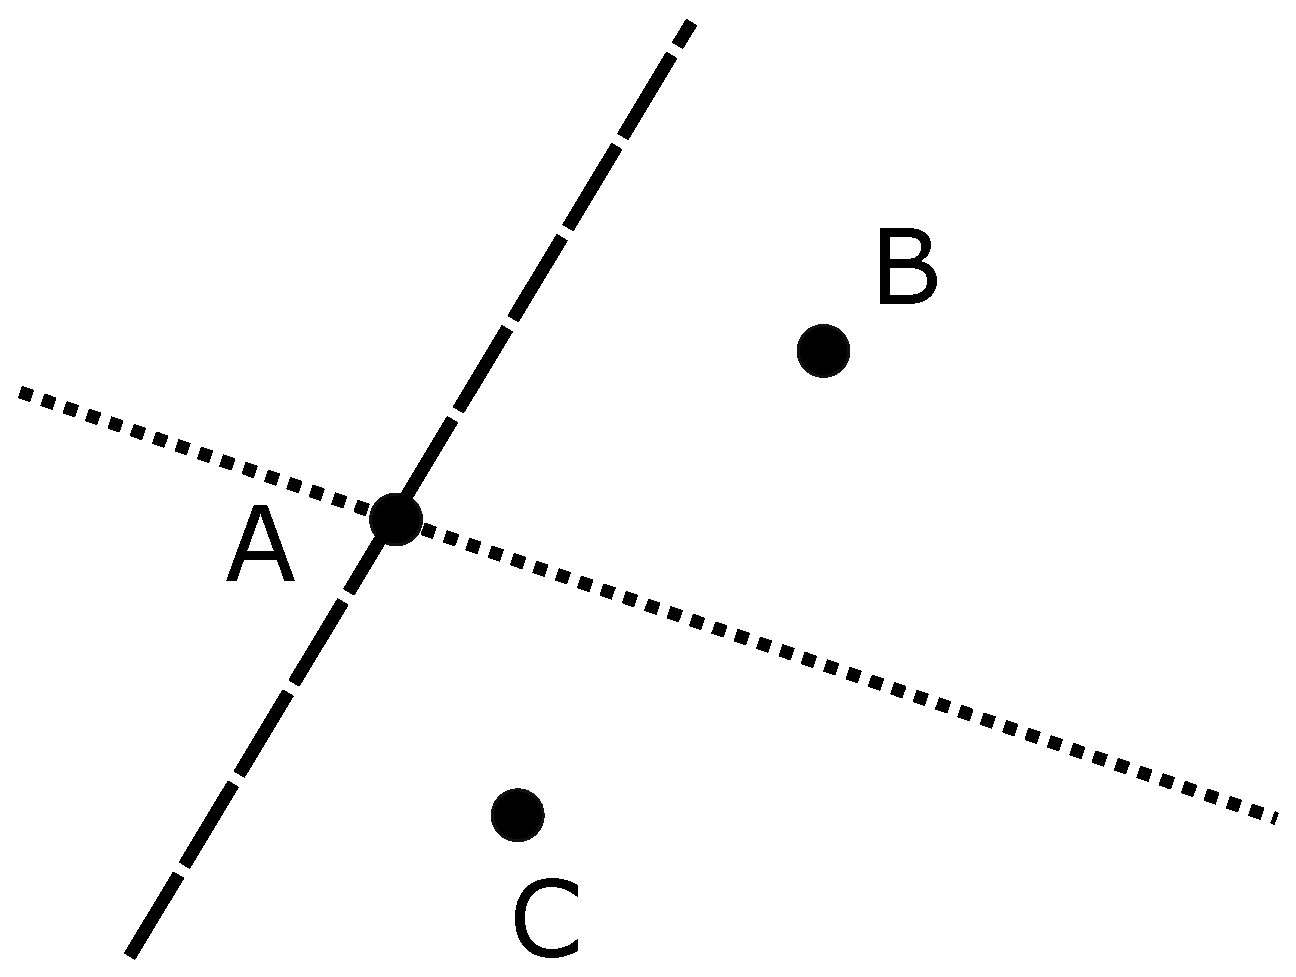
\includegraphics[width=0.5\textwidth]{5-19}
      
      \caption{Прямая, проходящая через точку $A$ и равноудалённая от точек $B$ и $C$.}
      \label{fig:5-19}
    \end{figure}
    
    Вместо (попыток) вычисления расстояний можно заметить, что нам подходят всего две прямые, которые определяются более ``дружелюбными'' условиями, с которыми уже можно будет работать.
    
    Так, первый случай~---~прямая $a$ параллельна $\bds{BC} \hm= (1 - 3, -1 - 7) \hm= (\textcolor{my-blue}{-2}, \textcolor{my-red}{-8})$ (\ref{fig:5-19}):
    \[
      a: \textcolor{my-red}{-8} x - \textcolor{my-blue}{(-2)} y + C = 0
    \]
    \[
      A \in a \Rightarrow -8 \cdot (-1) + 2 \cdot 5 + C = 0 \Rightarrow C = -18
    \]
    \[
      \boxed{4x - y + 9 = 0}
    \]
      
    Второй случай~---~когда прямая $a$ проходит между точками $B$ и $C$ (\ref{fig:5-19}).
    
    Пусть $M$~---~середина $BC$:
    $
      M = \left(\frac{1 + 3}{2}, \frac{-1 + 7}{2}\right) = (2, 3)
    $
    
    Прямая, проходящая через две точки $A(-1, 5)$ и $M(2, 3)$:
    \[
      \frac{x - x_M}{x_A - x_M} = \frac{y - y_M}{y_A - y_M}
      \Rightarrow
      \frac{x - 2}{-1 - 2} = \frac{y - 3}{5 - 3}
    \]
    \[
      \boxed{2x + 3y - 13 = 0}
    \]
  \end{solution}
  
  
  \subsection{\# 5.34(2) (р)}
  
  \begin{problem}
    Точка $A(1, 2)$ и прямая $a: 3x - y + 9 = 0$.
    Найти координаты
    \begin{enumerate}
      \item $A_{\perp}$~---~проекции $A$ на прямую $a$
      \item $A'$~---~точки, симметричной с $A$ относительно прямой $a$
    \end{enumerate}
  \end{problem}
  
  \begin{solution}
    Точка $A$ не лежит на прямой: $3 \hm\cdot 1 \hm- 1 \hm\cdot 2 \hm+ 9 \hm{\not=0}$
    
    Система прямоугольная $\Rightarrow \bds n \hm= (3, -1)$.
    
    $A_{\perp} \hm=(x, y)$, $A_{\perp} \in a$, $\vv{A_{\perp}A} \hm\parallel \bds n$:
    \[
      \left\{
        \begin{aligned}
          &3x - y + 9 = 0\\
          &\frac{1 - x}{2 - y} = \frac{x_A - x_{A_{\perp}}}{y_A - y_{A_{\perp}}} = \frac{n_x}{n_y} = \frac{3}{-1}
        \end{aligned}
      \right.
    \]
    \[
      \boxed{A_{\perp} = (-2, 3)}
    \]
    
    $A, A_{\perp}, A'$:
    \[
      \left\{\begin{aligned}
        &\vv{A A_{\perp}} = \vv{A_{\perp} A'}\\
        &\vv{A A_{\perp}} = (-2, 3) - (1, 2) = (-3, 1)
      \end{aligned}\right.
      \Rightarrow \vv{A_{\perp} A'} = (-3, 1)
    \]
    \[
      \vv{A_{\perp} A'} = A' - A_{\perp} \Rightarrow A' = \vv{A_{\perp} A'} + A_{\perp}
      = (-3, 1) + (-2, 3)
    \]
    \[
      \boxed{A' = (-5, 4)}
    \]
  \end{solution}
  
  
  \subsection{\# 5.54}
  
  \begin{problem}
    Составить уравнение биссектрисы острого угла между прямыми $l_1$ и $l_2$, заданными уравнениями:
    \[
      l_1\colon x - 7y - 1 = 0
    \]
    \[
      l_2\colon x + y + 7 = 0
    \]
  \end{problem}
  
  \begin{solution}
    Проверим сначала, что прямые в самом деле пересекаются.
    
    ...Это так, потому что коэффициенты $A$ и $B$ в уравнениях $l_1$ и $l_2$ не пропорциональны.
    
    Найдём же точку пересечения (почему нет).
    Эта точка~---~общая для двух прямых, то есть если обозначить её координаты как $(x^*, y^*)$, то они удовлетворяют уравнениям обеих прямых:
    \[
      \left\{
        \begin{aligned}
          &x^* - 7y^* - 1 = 0\\
          &x^* + y^* + 7 = 0
        \end{aligned}
      \right.
    \]
    
    Решая систему, получаем $(x^*, y^*) \hm= (-6, -1)$.
    
    Биссектрису вообще можно будет задать, если мы узнаем, например, какую-нибудь точку на биссектрисе и её направляющий вектор.
    Точка уже есть.
    Остался вектор.
    Его мы тоже сможем найти.
    
    Выберем сначала направляющие векторы прямых:
    \[
      \bds a_1 = (7, 1),\quad \bds a_2 = (-1, 1)
    \]
    
    (Видно, что прямые $l_1$ и $l_2$ не перпендикулярны, то есть в самом деле образуют острые и тупые углы в результате пересечения.)
    
    \begin{figure}[h]
      \centering
      
      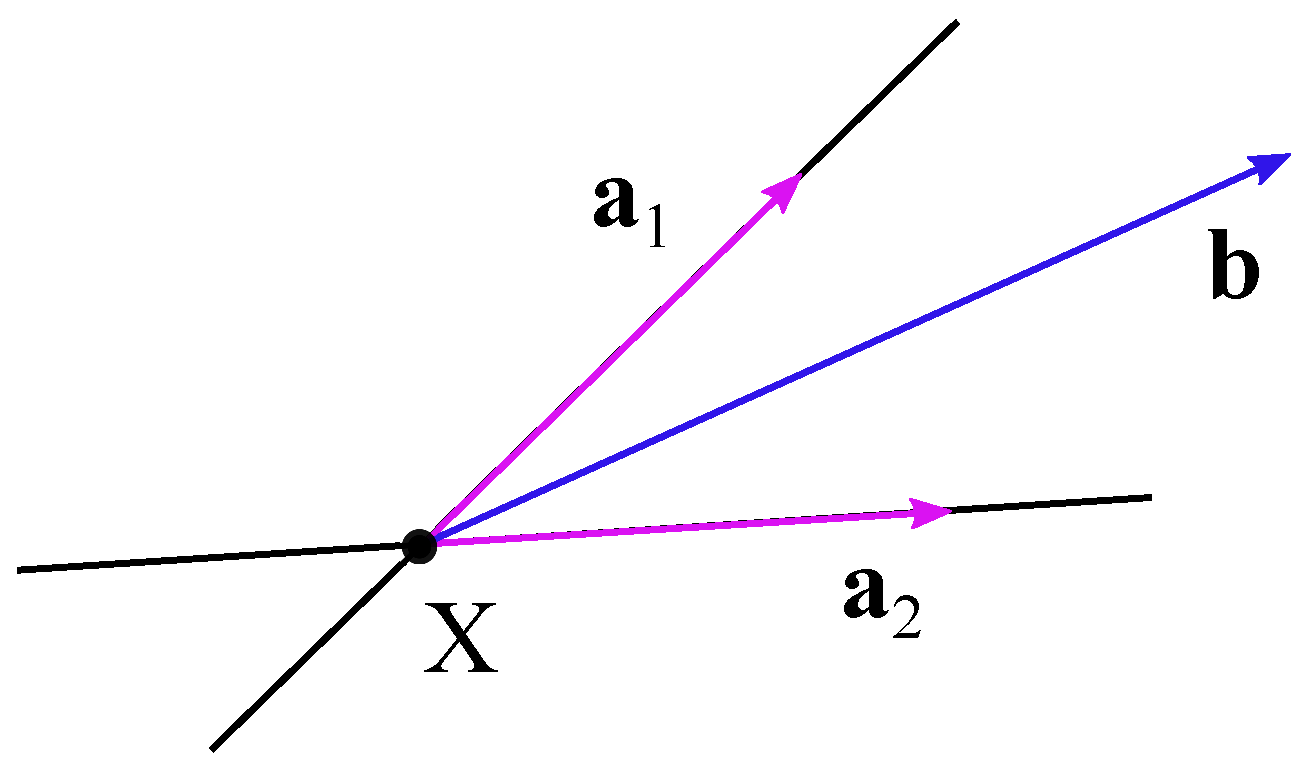
\includegraphics[width=0.5\textwidth]{5-54}
      
      \caption{Направляющий вектор $\bds b$ биссектрисы острого угла между $l_1$ и $l_2$.}
      \label{fig:5-54}
    \end{figure}
    
    ``Из геометрии'' не сложно видеть (\ref{fig:5-54}), что направляющий вектор биссектрисы $\bds b$ можно будет выбрать как сумму \emph{единичных по длине} направляющих векторов прямых $l_1$ и $l_2$, \emph{направленных вдоль сторон интересующего нас острого угла}.
    Векторы $\bds a_1$ и $\bds a_2$ можно будет отнормировать~---~это не проблема.
    Но образуют ли они острый угол?
    Проверим:
    \[
      (\bds a_1, \bds a_2) = 7 \cdot (-1) + 1 \cdot 1 < 0
    \]
    
    Нет.
    Тогда положим
    \[
      \bds a_1' \equiv -1 \cdot \bds a_1 = (-7, -1),\quad \bds a_2' \equiv \bds a_2 = (-1, 1)
    \]
    
    Проверим, что между такими векторами угол в самом деле будет острый:
    \[
      (\bds a_1', \bds a_2') = -7 \cdot (-1) - 1 \cdot 1 > 0
    \]
    
    Теперь отнормируем:
    \[
      \bds a_1'' \equiv \frac{\bds a_1'}{|\bds a_1'|} = \frac{1}{5\sqrt{2}} \begin{pmatrix}
        -7 \\ -1
      \end{pmatrix}
    \]
    \[
      \bds a_2'' \equiv \frac{\bds a_2'}{|\bds a_2'|} = \frac{1}{\sqrt{2}} \begin{pmatrix}
        -1 \\ 1
      \end{pmatrix}
    \]
    
    Наконец можем определить направляющий вектор биссектрисы:
    \[
      \bds b = \bds a_1'' + \bds a_2'' = \frac{4}{5 \sqrt{2}} \begin{pmatrix}
        -3 \\ 1
      \end{pmatrix}
    \]
    
    Векторное параметрическое уравнение биссектрисы острого угла:
    \[
      \bds r = \begin{pmatrix}
        -6 \\ -1
      \end{pmatrix} + \frac{4}{5 \sqrt{2}} \begin{pmatrix}
        -3 \\ 1
      \end{pmatrix} t,\quad t \in \RR
    \]
    
    Можно переписать его в более ``простом'' виде~---~чтоб можно было сравнить с ответом в конце задачника :)
    \[
      \frac{x - (-6)}{y - (-1)} = \frac{-3}{1} \Leftrightarrow x + 3y + 9 = 0
    \]
  \end{solution}
  
  
  %\subsection{\# 5.61}
  %
  %\begin{problem}
    %Найти радиус и координаты центра окружности, проходящей через точку А и касающейся двух прямых.
  %\end{problem}
  %
  %\begin{solution}
    %Центр окружности~---~на биссектрисе.
    %P.S. Система координат прямоугольная.
  %\end{solution}
  
  
  \section{Дополнение 1: ``Другое решение другой задачи''}
  
  \subsection{\# 5.53 (р)}
  
  \begin{problem}
    Две прямые: $x - 7y = 1$ и $x + y \hm= -7$.
    Уравнение биссектрисы угла с точкой $A(1, 1)$ внутри?
  \end{problem}
  
  \begin{solution}
    \emph{Изложенное далее отличается от решения в задачнике.
    Возможно, вариант, представленный здесь, менее рациональный, но всё же, хочется думать, тоже небесполезный.}
    
    Прямые пересекаются, точка $A$ не лежит ни на одной прямой.
      
    Точка пересечения прямых $X(x, y)$:
    \[
      \left\{\begin{aligned}
        &x - 7y = 1\\
        &x + y = -7
      \end{aligned}\right.
      \Rightarrow
      \left\{\begin{aligned}
        &x = -6\\
        &y = -1
      \end{aligned}\right.
    \]
    \[
      \boxed{X = (-6, -1)}
    \]
    
    \begin{figure}[h]
      \centering
      
      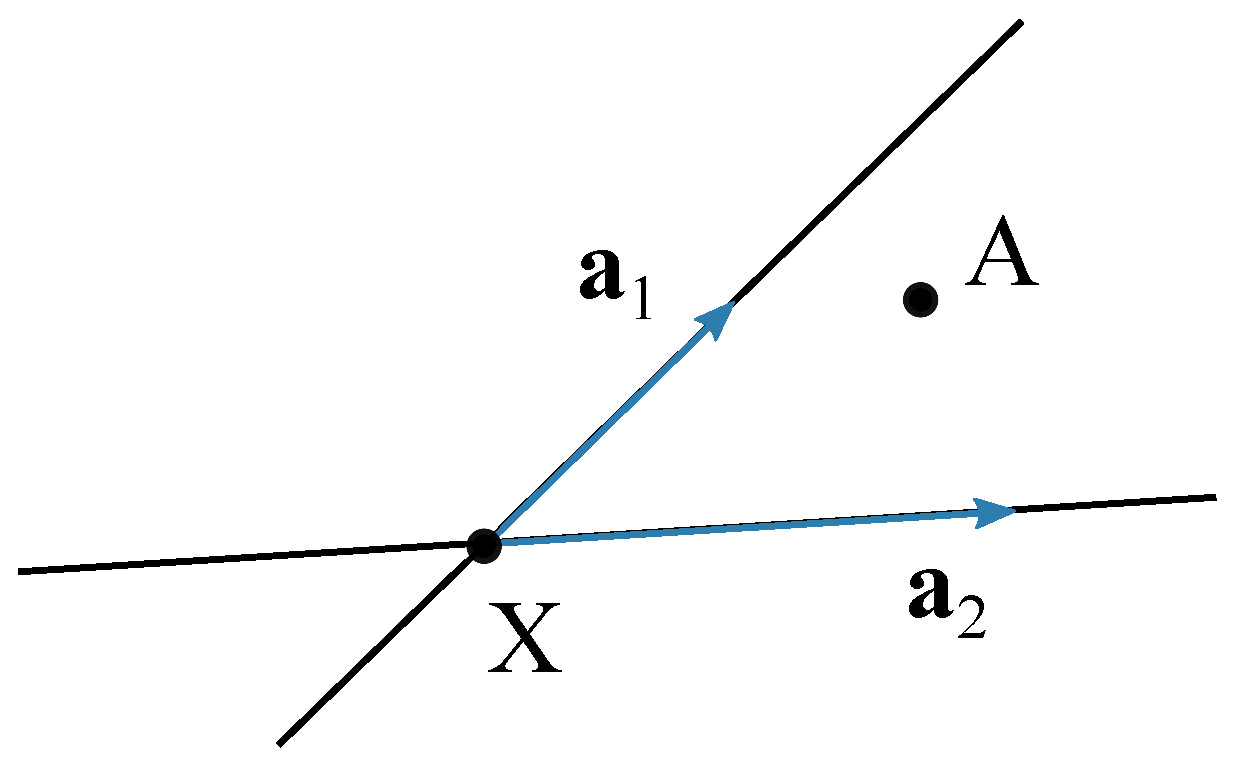
\includegraphics[width=0.5\textwidth]{5-53}
      
      \caption{Точка $A$ лежит внутри угла, образованного векторами $\bds a_1$ и $\bds a_2$, отложенными от точки $X$.}
      \label{fig:5-53}
    \end{figure}

    Выберем направляющие векторы прямых $\bds a_1$, $\bds a_2$ так, чтобы они образовывали угол с точкой $A$ внутри (\ref{fig:5-53}).
    \[
      [\bds a_i, \vv{XA}] = \left|
        \begin{aligned}
          &\bds i & &\bds j & &\bds k\\
          &a_{ix} & &a_{iy} & &0\\
          &XA_x & &XA_y & &0
        \end{aligned}
      \right|
      = \bds k \cdot (a_{ix} \cdot XA_y - XA_x \cdot a_{iy})
    \]
    \[
      \vv{XA} = (1, 1) - (-6, -1) = (7, 2)
    \]
    \[
      \bds a_1 = (7, 1) \Rightarrow \sgn{(7 \cdot 2 - 7 \cdot 1)} = +
    \]
    \[
      \bds a_2 = (-1, 1) \Rightarrow \sgn{(-1 \cdot 2 - 7 \cdot 1)} = -
    \]
    
    Получаем, что при выбранных $\bds a_1$ и $\bds a_2$ направление поворота от $\bds a_1$ к $\vv{XA}$ по наименьшему углу не совпадает с направлением поворота от $\bds a_2$ к $\vv{XA}$ по наименьшему углу.
    То есть $A$ лежит внутри угла, образованного $\bds a_1$ и $\bds a_2$, отложенными из точки $X$.
    Итак, полагаем
    \[
      \boxed{\bds a_1 \equiv (7, 1),\ \bds a_2 \equiv (-1, 1)}
    \]

    Пусть $\bds b \hm= (b_x, b_y)$~---~направляющий вектор биссектрисы. Точки на биссектрисе равноудалены от сторон угла:
    \[
      \frac{(\bds a_1, \bds b)}{|\bds a_1||\bds b|} = \cos \angle (\bds a_1, \bds b)
      = \cos \angle (\bds a_2, \bds b)
      = \frac{(\bds a_2, \bds b)}{|\bds a_2||\bds b|}
    \]
    \[
      \frac{7 b_x + b_y}{|\bds a_1|} = \frac{-b_x + b_y}{|\bds a_2|}
      \Rightarrow
      \bds b = \bigl(|\bds a_1| - |\bds a_2|, 7|\bds a_2| + |\bds a_1|\bigr)
    \]
    \[
      |\bds a_1| = \sqrt{50},\ |\bds a_2| = \sqrt{2} \Rightarrow \bds b = (5 - 1, 7 + 5) = (4, 12)
    \]

    Уравнение биссектрисы:
    \[
      \frac{x - (-6)}{4} = \frac{y - (-1)}{12}
      \Rightarrow \boxed{3x - y + 17 = 0}
    \]
  \end{solution}
  
  
  \section{Дополнение 2: Пара задач про прямую в пространстве}
  
  \subsection{\# 6.3}
  
  \begin{problem}
    При каком необходимом и достаточном условии прямые $\bds r \hm= \bds r_1 + \bds a_1 t$ и $\bds r \hm= \bds r_2 \hm+ \bds a_2 t$
    \begin{itemize}
      \item Пересекаются в единственной точке?
      \item Скрещиваются?
      \item Параллельны, но не совпадают?
      \item Совпадают?
    \end{itemize}
  \end{problem}
  
  \begin{solution}
    \begin{figure}[h]
      \centering
      
      \includegraphics[width=0.5\textwidth]{lines-in-3d}
      
      \caption{Варианты взаимного расположения двух прямых в пространстве.}
      \label{fig:lines-in-3d}
    \end{figure}
    
    Решение этой задачи отчасти похоже на решение для случая $2$D.
    Снова рассмотрим пункты по порядку (\ref{fig:lines-in-3d}).
    
    \begin{enumerate}
      \item В пространстве уже недостаточно только лишь неколлинеарности $\bds a_1$ и $\bds a_2$.
      Надо ``отсечь'' случай, когда прямые скрещиваются.
      То есть надо потребовать, чтобы прямые лежали в одной плоскости.
      Для этого необходимо и достаточно, чтобы четыре точки: две на одной прямой, и две на другой~---~лежали в одной плоскости (прямая определяется по двум точкам, плоскость по трём).
      На первой прямой можно взять точки $\bds r_1$, $\bds r_1 \hm+ \bds a_1$.
      На второй~---~точки $\bds r_2$, $\bds r_2 \hm+ \bds a_2$.
      Чтобы проверить, что четыре точки лежат на одной плоскости, можно построить три вектора с началом в одной из четырёх точек и концами в оставшихся трёх.
      Например, можно рассмотреть векторы $\bds r_1 \hm- \bds r_2$, $\bds r_1 \hm+ \bds a_1 \hm- \bds r_2$ и $\bds r_2 \hm+ \bds a_2 \hm- \bds r_2 \hm= \bds a_2$ (откладываем векторы от точки $\bds r_2$).
      Далее на получившихся трёх векторах можно построить параллелепипед и посчитать его объём: если он больше нуля, то исходные четыре точки не лежат на одной плоскости, если равен нулю~---~то лежат.
      Объём же можно посчитать с помощью смешанного произведения (сначала в формуле под векторами имеются в виду направленные отрезки, при появлении же определителя под векторами понимаются столбцы из компонент векторов в некотором правом ортонормированном базисе):
      \begin{equation*}
      \begin{split}
        V_{\pm} &= (\bds r_1 - \bds r_2, \bds r_1 + \bds a_1 - \bds r_2, \bds a_2)\\
        &= \bigl|(\bds r_1 - \bds r_2, \bds r_1 + \bds a_1 - \bds r_2, \bds a_2)^T\bigl|
        = \Bigl|\bigl(\bds r_1 - \bds r_2, \bds a_1 + (\bds r_1 - \bds r_2), \bds a_2\bigr)^T\Bigl|
        = \bigl|(\bds r_1 - \bds r_2, \bds a_1, \bds a_2)^T\bigl|
      \end{split}
      \end{equation*}
      где в последнем переходе использовалось свойство определителя, заключающееся в том, что к любой строке (или столбцу) можно прибавлять линейную комбинацию остальных строк (или столбцов)~---~при этом определитель не меняется.
      В случае $3$D первое условие (неколлинеарность $\bds a_1$ и $\bds a_2$) можно записать ещё и с помощью векторного произведения.
      Итого, получаем два условия
      \[
        \left\{
          \begin{aligned}
            &[\bds a_1, \bds a_2] \not= \bds 0\\
            &(\bds r_1 - \bds r_2, \bds a_1, \bds a_2) = 0
          \end{aligned}
        \right.
      \]
      
      \item Получается из предыдущего пункта заменой одного условия на противоположное (условия, с помощью которого разделяли случаи скрещивания и собственно пересечения):
      \[
        \left\{
          \begin{aligned}
            &[\bds a_1, \bds a_2] \not= \bds 0\\
            &(\bds r_1 - \bds r_2, \bds a_1, \bds a_2) \not= 0
          \end{aligned}
        \right.
      \]
      
      \item Параллельны~---~условие $\bds a_1 \hm\parallel \bds a_2$.
      Не совпадают~---~так же, как и в $2$D (так как параллельные прямые лежат в одной плоскости).
      То есть $(\bds r_1 \hm- \bds r_2) \hm{\not\parallel} \bds a_1$.
      И получаем
      \[
        \left\{
          \begin{aligned}
            &[\bds a_1, \bds a_2] = \bds 0\\
            &[\bds r_1 - \bds r_2, \bds a_1] \not= \bds 0
          \end{aligned}
        \right.
      \]
      
      \item Получается из предыдущего заменой одного условия на противоположное:
      \[
        \left\{
          \begin{aligned}
            &[\bds a_1, \bds a_2] = \bds 0\\
            &[\bds r_1 - \bds r_2, \bds a_1] = \bds 0
          \end{aligned}
        \right.
      \]
    \end{enumerate}
  \end{solution}
  
  
  \subsection{\# 6.1(2, 3, 5)}
  
  \begin{problem}
    Для прямой, заданной одним уравнением, записать её же уравнение, но в другой форме.
    \begin{enumerate}
      \setcounter{enumi}{1}
      
      \item $\bds r = \bds r_0 + \bds a t \xrightarrow{\?} [\bds r, \bds a] = \bds b$
      
      \item $[\bds r, \bds a] = \bds b \xrightarrow{\?} \bds r = \bds r_0 + \bds a t$
      
      \setcounter{enumi}{4}
      
      \item $\left\{
        \begin{aligned}
          &(\bds r, \bds n_i) = D_i\\
          &i = 1, 2
        \end{aligned}
      \right. \xrightarrow{\?} \bds r = \bds r_0 + \bds a t$
    \end{enumerate}
  \end{problem}
  
  \begin{solution}
    Пойдём по по пуктам по порядку.
    
    \begin{enumerate}
      \setcounter{enumi}{1}
      
      \item
        \[
          \bds r - \bds r_0 = \bds a t
          \Leftrightarrow (\bds r - \bds r_0) \parallel \bds a
          \Leftrightarrow [\bds r - \bds r_0, \bds a] = \bds 0
        \]
        \[
          [\bds r, \bds a] = [\bds r_0, \bds a] \equiv \bds b
        \]
      
      \item
        \[
          [\bds a, \bds b] = \bds a \times (\bds r \times \bds a) = \bds r (\bds a \cdot \bds a) - \bds a (\bds a \cdot \bds r)
        \]
        \[
          \bds r = \frac{[\bds a, \bds b]}{|\bds a|^2} + \bds a \cdot \left(\frac{\bds a}{|\bds a|^2} \cdot \bds r\right)
          = \bds r_0 + \bds a t
        \]
        где $\bds r_0 \hm\equiv \dfrac{[\bds a, \bds b]}{|\bds a|^2}$ и $t \hm\equiv \left(\dfrac{\bds a}{|\bds a|^2} \cdot \bds r\right)$.
      
      \setcounter{enumi}{4}
      
      \item
        Направляющий вектор прямой $\bds a$ можно найти как
        \[
          \bds a = [\bds n_1, \bds n_2]
        \]
        (при этом $\bds n_1$ и $\bds n_2$ не должны быть коллинеарны, иначе пара плоскостей не задаёт одну прямую).
        Остаётся найти начальный вектор прямой $\bds r_0$.
        Он удовлетворяет обоим уравнениям плоскостей
        \[
          \left\{
          \begin{aligned}
            &(\bds r_0, \bds n_1) = D_1\\
            &(\bds r_0, \bds n_2) = D_2
          \end{aligned}
          \right.
        \]
        Скалярные произведения $\bds r_0$ на векторы нормали $\bds n_i$~---~первые две компоненты вектора $\bds r_0$ в базисе, взаимном к, например, $\bds n_1$, $\bds n_2$, $\bds a$.
        Будем искать $\bds r_0$ такой, что он лежит в плоскости, перпендикулярной искомой прямой (то есть вектору $\bds a$).
        Тогда третья компонента во взаимном базисе $(\bds r_0, \bds a) \hm= (\bds r_0, [\bds n_1, \bds n_2]) \hm= 0$.
        
        Выпишем вектора взаимного базиса:
        \[
          \left\{
          \begin{aligned}
            &\bds e_1^* = \frac{[\bds n_2, \bds a]}{(\bds n_1, \bds n_2, \bds a)} = \frac{|\bds n_2|^2}{|\bds n_1|^2 \cdot |\bds n_2|^2} \cdot \bds n_1\\
            &\bds e_2^* = \frac{[\bds a, \bds n_1]}{(\bds n_1, \bds n_2, \bds a)} = \frac{|\bds n_1|^2}{|\bds n_1|^2 \cdot |\bds n_2|^2} \cdot \bds n_2\\
            &\bds e_3^* = \frac{[\bds n_1, \bds n_2]}{(\bds n_1, \bds n_2, \bds a)} = \frac{1}{|\bds n_1|^2 \cdot |\bds n_2|^2} \cdot \bds a
          \end{aligned}
          \right.
        \]
        (смешанное произведение $(\bds n_1, \bds n_2, \bds a)$ можно посчитать через ``бац минус цаб''; а третий вектор $\bds e_3^*$ можно было и не выписывать).
        
        Поэтому для $\bds r_0$ получаем
        \[
          \bds r_0
          = D_1 \cdot \frac{|\bds n_2|^2}{|\bds n_1|^2 \cdot |\bds n_2|^2} \bds n_1 + D_2 \cdot \frac{|\bds n_1|^2}{|\bds n_1|^2 \cdot |\bds n_2|^2} \bds n_2
          = \frac{D_1}{|\bds n_1|^2} \bds n_1 + \frac{D_2}{|\bds n_2|^2} \bds n_2
        \]
        
        И итоговое уравнение прямой
        \[
          \bds r = \left(\frac{D_1}{|\bds n_1|^2} \bds n_1 + \frac{D_2}{|\bds n_2|^2} \bds n_2\right) + [\bds n_1, \bds n_2] \cdot t
        \]
        
        \bigskip
        
        \emph{Дополнение.}
        
        Автор конспекта точно не знает, можно ли из уравнения прямой на плоскости $(\bds r, \bds n) \hm= D$ получить векторное параметрическое уравнение $\bds r \hm= \bds r_0 \hm+ \bds a t$.
        Скорее всего, нельзя, потому что нет возможности на плоскости с помощью рассмотренных операций получить из вектора $\bds n$ вектор, ему перпендикулярный.
        Но начальную точку на прямой найти можно:
        \[
          (\bds r_0, \bds n) = D
        \]
        И, как и раньше, полагая $\bds r_0$ перпендикулярным прямой (то есть параллельным $\bds n$), получаем
        \[
          \bds r_0 = \alpha \bds n
          \Rightarrow \alpha (\bds n, \bds n) = D
          \Rightarrow \alpha = \frac{D}{(\bds n, \bds n)} = \frac{D}{|\bds n|^2} 
          \Rightarrow \boxed{\bds r_0 = \frac{D}{|\bds n|^2} \bds n}
        \]
    \end{enumerate}
  \end{solution}
\end{document}
